\chapter{Preliminary Material }

\section{General}
\begin{enumerate}


\item Always true, sometimes true or never true:  If $a$ is a real number, then $$\sqrt {a^2 }  = a.$$

\item Decide if the following statements are always true or not?  Are there special cases?  If a statement is not always true, can you change the equation to an inequality so that it is true.  Explain why the inequality is true.    $$\left| {ab} \right| = \left| a \right|\left| b \right|$$  $$\left| {a + b} \right| = \left| a \right| + \left| b \right|$$

\item Define a logarithm.  Explain the relationship between logarithmic and exponential functions.  What do logarithms give the ability to do?  

\item Explain the difference between the terms positive and nonnegative.  Give examples using both interval notation and numbers lines.  What terms would we use to describe the sets $(-\infty, 0)$ and $(-\infty, 0]$?

\item Explain what is meant by $(-\infty, 7]$.

\item How do you know that $${{x^2  + y^2 } \over {\left( {x + y} \right)^2 }} \ne 1? \cite{B}$$  

\item In which formulas do the increments $\Delta x$ and $\Delta y$ show up?  Give a graphical representation of what the $\Delta x$ and $\Delta $y represent in each formula.  

\item Investigate the validity of this statement:  If $f(x)$ and $g(x)$ are functions, then $$f \circ g\left( x \right) = g \circ f\left( x \right).$$

\item Look back at the homework and writing assignments you have done so far and identify concepts that you feel you know the best.  Identify areas that you need to improve on before the exam.  If you could improve on one concept before the exam, what concept would be the most beneficial to you and why? Which are the trickiest? 


\item Suppose a friend has dug holes for the corner posts of a rectangular deck.  Explain how to use the Pythagorean Theorem to test whether or not the holes form a rectangle.  \cite{SM} 

\item Suppose that $y$ is measured in feet and $x$ is measured in seconds.  What are the dimensions of the constants $a$, $b$, $c$ and $d$ in the function $$y = ax^3  + bx^2  + cx + d?$$

\item The absolute value of $x$ is defined to be $$
\left| x \right| = \left\{ \matrix{
  x\ \ {\rm{ for }}\ \ x \ge 0 \hfill \cr 
  x\ \ {\rm{ for }}\ \ x < 0 \hfill \cr}  \right.  .
$$
  To understand this definition, you must believe that $$\left| x \right| =  - x$$ for negative values of $x$.  Using $x = -3$ as an example, explain why $-x = (-1)x$ produces the same result as taking the absolute value of $x$.  \cite{SM}

\item The rules of exponents tell us that $a^0 = 1$ if $a$ is any number different from zero.  The also tell us that $0^n = 0$ if $n$ is any positive number.  Neither definition tells us the value of $0^0$.  We will learn later that this is called an indeterminate form.  If we follow the first rule (i.e., $a^0 = 1$) we get $0^0 = 1$.  If we follow the second rule (i.e., $0^n = 0$) we get $0^0 = 0$.  The rules of mathematics are designed to be consistent which explains why $a = 0$ is excluded from the first rule and $n = 0$ is excluded from the second rule.\\We are not dealing with a question of right or wrong here.  Neither rule applies as it stands, so there is no contradiction.  What value would you like $0^0$ to have?  If we chose a value we might want it to make functions that evaluate to $0^0$ continuous because we like continuous functions.  Consider the following examples.\\a)  
Calculate $x^x$ for $x$ = 0.1, 0.001, 0.0001, and so on as far as your calculator will go.  What pattern do you see?\\b)  As $x$ increases without bound, $1/x$ approaches 0.  As $x$ increases without bound, $1/\ln x$ approaches 0.  So, as $x$ increases without bound, $$f(x) = \left( {{1 \over x}} \right)^{{\textstyle{1 \over {\ln x}}}} $$ approaches $0^0$.  What value would we like to give this function as $x$ increases without bound?  Evaluate $f$ for $x$ = 10, 100, 1000 and so on as far as your calculator can reasonable go.  What pattern do you see. \\ c)  What does this say about possible values of $0^0$?  \cite{FWG}

\item We often write ``$-4 < x < 4$'' in place of ``$-4 < x$ and $x < 4$''.  Unfortunately, many people write ``$4 < x < -4$'' in place of ``$4 < x$ or $x > -4$''.  Explain why  ``$4 < x < -4$'' could never be true.  \cite{SM}



\item Write a formal definition of these terms and then explain them in every day language:  circle, angle of inclination of a line, function, domain, and range.

\item Write up to 5 distinct questions that I might ask on an exam about the following information:    $
P_1 \left( {3, - 2} \right)
$ and $P_2 \left( { - 3,5} \right)$
.


\item Write up to 5 distinct questions that I might ask on an exam about the following information:  $3x + 2y = 6$.

\item Write up to 5 distinct questions that I might ask on an exam about the following information:  $x^2 - 2x$.

\item Investigate the validity of this statement:  $e = 2.71828.$

\item Explain the connection between completing the square and the quadratic formula.  

\item Is $0^r = 0$ for any value of $r$?  Try these values before making your decision:  $r = 2$, ${\textstyle{1 \over 2}},$ 1000, $-2$, $ - {\textstyle{3 \over 2}},$ 0.15 and 0.

\end{enumerate}

\section{Solving Equations}
\begin{enumerate}

\item You and a friend are working on some calculus homework and in the process of doing one of the problems, you have to solve this equation:
		 \begin{equation}
6 = c\left( {c - 4} \right)
.\label{AAA}\end{equation}
Your friend says that you can solve by setting each factor each to 6, and solving each equation, like this:$$
\begin{array}{clcl}
   &6 = c& {\rm{ and }}& 6 = c - 4  \\
   {\rm{so }}&c = 6& {\rm{ and }}& c = 10. \\ 
\end{array}$$	 
Using some numbers, explain to your friend why this won't work for Equation \ref{AAA} but it will work for 
		 $$
0 = c\left( {c - 4} \right).
$$
Then, show your friend how to solve Equation \ref{AAA} using the quadratic formula.

\item a)  Solve the equation $$e^x  + e^{ - x}  = 5$$ by following these steps.  First, make a substitution $u = e^x .$  Note that $e^{ - x}  = {1 \over {e^x }}.$  Now, clear the fractions and you should recognize how to solve this equation for $u$.  Finally, now that you know the value of $u$, solve for $x$ in $u = e^x .$  (Don't forget that $e^x$ is always positive.) \\  b)  To practice your new found skill, solve $2^x  - 2^{ - x}  = 3$ for $x$.

\item Solve each of the following 2 quadratic equations (giving exact values).  Justify the methods you used to solve each equation.  $$x^2 - 2x = 0$$ $$x + x^2 = 2$$

\item What do the following 6 questions have in common?
\begin{enumerate}\item  Find the zeros of $f(x) = x^3 - 3x - 1$.
\item  Find the $x$-coordinates of the points where the curve $y = x^3$  crosses the line $y = 3x + 1$.
\item Find the values of $x$ for which $x^3 - 3x = 1$.
\item  Find the $x$-values where the curve $y = x^3 - 3x$ intersects the vertical line through $(0, 1)$.
\item Solve the equation $x^3 - 3x - 1 = 0$.
\item  Find the $x$-intercepts of $f(x) = x^3 - 3x - 1$.
\end{enumerate}

\end{enumerate}

\section{Slopes and Equations of Lines} 
\begin{enumerate}

\item There are four forms of linear equations.  What are they?  Discuss the advantages and disadvantages of each one.  Also, describe how each holds up under the special cases of horizontal and vertical lines.

\item What are the units of the slope of line if the units of $x$ are seconds and the units of $y$ are feet?  Complete a dimensional analysis of $y = mx + b$.  

\item If the slope between points $A$ and $B$ equals the slope between points $B$ and $C$, explain why the points $A$, $B$, and $C$ are collinear.  \cite{SM} 

\item A friend of yours in class did the following work.     
 $$P_1 \left( {3, - 2} \right)  \ \ \ \ \ P_2 \left( { - 3,5} \right)  $$ 
$$m = {{5 - ( - 2)} \over {3 - ( - 3)}} = {7 \over 6} $$
   
 Gently and correctly, explain to your friend what their mistake is and give them pointers for organizing their work so they can avoid this error in the future.

\item Find the equation of the bisector of the acute angle between $x + y - 4 = 0$ and    $x - 7y + 2 = 0$.  

\item How would you define the distance from a point to a line?  Draw a picture to illustrate what you mean and check with others in the class before continuing.  Let $(a, b)$ be the point and $Ax + By = C$ be the line.  Derive the formula for the distance from $(a, b)$ to $Ax + By = C$ by doing the following:    \\a)  Find the slope of the line from $(a, b)$ to the line $Ax + By = C$ that you are going to measure the distance along.    \\b)  Find the equation of the line you are going to measure along.    \\c)  Find the point where $Ax + By = C$ intersects the line you found in part b).    \\d)  Find the distance from point $(a, b)$ to the point you found.    \\e)  Create an example to illustrate the formula you just created.

\item Consider the following list of lines.  Sort this list in a way that shows which lines are parallel to each other and which are perpendicular to each other.  After the sorting, explain the process you used for determining which lines were parallel and which were perpendicular.  An important aspect of this problem is how you choose to organize your solution.      
$$\matrix{   
y = {1 \over 3}x + 5 & 
		{1 \over x} + {3 \over y} = 0 & 
		3x - y = 10 & 
			2x = 6y + 1  \cr \cr   
2x = 3y & 
		3\left( y - 2 \right) = x & 
		2x = 3y & 
		3y = 2x + 1  \cr \cr   
x = 3y & 
	{1 \over 2}x + {1 \over 3}y = 2 & 
	3\left( x - 2 \right) = 2\left( y + 1 \right) & 
	3x + 2y + {2 \over 3} = 0  \cr  \cr  
x + 3y = 0 & 
	2\left( x - 2 \right) + 3\left( y + 1 \right) = 0 & 
	2x = 3y & 
	{1 \over 3}x = {1 \over 2}y - 7.2  \cr  } $$

\item Given 2 points in the plane, what is your preferred method for finding the equation of a line that passes through those 2 points?  First, describe your method in general.  Then, make up an example using your method and annotate it. 

\item Find the equation of the line that passes through the points where $x^2 - 4x + y^2 + 2y - 4 = 0$ and $x^2 - 10x + 20 + y^2 - 4y = 0$ intersect.  

\item Find the equation of the perpendicular bisector of the line segment joining $(2, 2)$ and     $(5, -1)$.  

\item If the points $(2, 4)$ and $(-1, 6)$ are on the line $L$, find another point on $L$.  

\end{enumerate}

\section{Functions and Graphs}

\begin{enumerate}

\item In Figure \ref{Chapter1Figureb}  is the graph of the function $f(t)$ that represents your height about ground at time $t$.  Write an explanation of what you are doing to make the graph look like it does.  \cite{MR}   %put Chapter 1 Figure b here

\begin{figure}[ht]
	\centering
		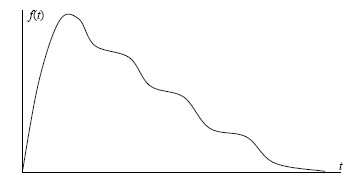
\includegraphics{TeXGraphics/Chapter1b.jpg}
	\caption{Height versus time}
	\label{Chapter1Figureb}
\end{figure}

\item In Figure \ref{Chapter1Figurec} is the graph of the function $g(t)$ that represents your distance from dorm room at time $t$.  Write an explanation of what you are doing to make the graph look like it does.%put Chapter 1 Figure b here

\begin{figure}[ht]
	\centering
		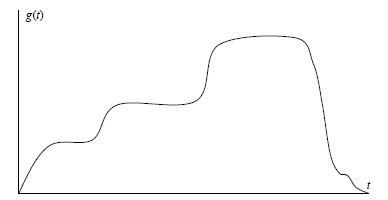
\includegraphics{TeXGraphics/Chapter1c.jpg}
	\caption{Distance from dorm room versus time}
	\label{Chapter1Figurec}
\end{figure}

\item The vertical line test provides a graphical way of determining whether a graph is a function or not.  Explain the vertical line test verbally and analytically. 

\item Consider the following forms of a quadratic function.    $$f(x) = a(x - b)(x - c)$$  $$f(x) = a(x - d)^2 + g$$  $$f(x) = ax^2 + bx + c$$    Discuss the advantages and disadvantages of each one. 

\item First, graph $$f(x)=(x-1)(x+2)(x-3)(x+4).$$  To practice using interval notation, find the intervals where $f(x)$ is positive and the intervals where $f(x)$is negative.  Explain how to do this to a friend that missed class that day.

\item Starting from a single cell, a human being is formed by 50 generations of cell division.  Explain why after $n$ divisions there are $2^n$ cells.  Guess how many cells will be present after 50 divisions.  Now compute $2^{50}$ and compare to your guess.  Briefly discuss how rapidly exponential functions increase.  \cite{SM}

\item Are there 2 functions $f$ and $g$ such that $f \circ g = g \circ f?\ \ \cite{FWG}$    

\item Are there 2 functions $f $ and $g$ such that the graphs of $f$ and $g$ are not straight lines but the graph $f \circ g$ is a straight line?  \cite{FWG}

\item If $f(x)$ is odd can anything be said of $g(x) = f(x) - 2$? If $f(x)$ is even can anything be said of $g(x) = f(x) - 2$?  \cite{FWG}

\item Explain why the graphs of $f(x) = 2^{ - x}$  and $ g(x) = \left( {{\textstyle{1 \over 2}}} \right)^x $ are the same.  \cite{SM}

\item Define a function and give examples of functions and non-functions explaining each example.

\item Give examples of each of the following functions and explain how to identify each one.  Explain how to find the domains in each class of functions.     \\   linear, constant, radical, rational, quartic, exponential

\item Describe in everyday language what the graphs of even and odd functions look like?  Explain that even and odd functions are not opposite concepts by doing the following.    \\a)  Draw a graph of a function that is neither even nor odd.    \\b)  Draw a graph of a function that is odd but not even.    \\c)  Draw a graph of a function that is even but not odd.    \\d)  Draw a graph of a function that is both even and odd.

\item Can a linear function be odd?  Can a linear function be even? 

\item a)  Can a function have more than one $x$-intercept?     \\b)  Can a function have more than one $y$-intercept?     \\c)  What do the intercepts say about the graph of a function?

\item a)  Explain why $c$ and $d$ are the $x$-intercept and $y$-intercept, respectively, of $${x \over c} + {y \over d} = 1.$$    \\b)  How are the $x$-intercept and $y$-intercept related to $c$ and $d$ in $${x \over c} + {y \over d} = 2.\ \   \cite{FWG}  $$  \\c)  Generalize.  

\item If $$f(x) = {1 \over {x + 1}},$$ what value(s) of $x$ satisfy $$f\left( {{1 \over {x + 1}}} \right) = f\left( {{{2x + 1} \over {2x + 4}}} \right).$$

\item Explain how to find the solution to $${{x - 2} \over {x + 1}} > 0$$ from the graph of $$f(x) = {{x - 2} \over {x + 1}}.$$  Describe this in a general way in order to help someone solve rational inequalities in general.

\item Choose some numbers in the domain of $$f(x) = {{\sqrt {x^2  - 1} } \over {x^2  - x - 6}}.$$  Choose some numbers that are not in the domain.  How did you find these numbers?

\item Investigate the validity of this statement:  The only graphs that are functions are those that are defined by a specific equation $y = f(x)$.

\item Explain the process of using your calculator to graph all of the circle $x^2 + y^2 = 4$.  

\item Discuss the issues of finding the domain of $f(x) = \left( {2x - 1} \right)^{ - {3 \mathord{\left/ {\vphantom {3 2}} \right. \kern-\nulldelimiterspace} 2}} .$

\item What does ``inverse'' mean?  What is an inverse function?  What are the inverse functions for each of the following?  Why is an inverse function useful?      $$\matrix{f(x) = x + 3&g(x) = 2x &h(x) = {1 \over x}\cr \cr k(x) = \sqrt x &j(x) = e^x &l(x) = \sin x\cr}$$  

\item Most of the time in mathematics, the notation we use is consistent.  However, there are times when it is not.  In particular, we use a superscript``$-1$'' to mean 2 different things.  Explain the difference in the meaning of $$x^{ - 1} \ \  {\rm{and}}\ \  \sin ^{ - 1} x.$$  What do each of these represent, how are each of these used, and how is the representation different for each?  Give other examples of the use of each notation and explain which of $$x^{ - 1} \ \  {\rm{and}}\ \  \sin ^{ - 1} x$$ each usage is like.

\item How do we prove that one function is the inverse of the other?  Why does this ``proof'' work, i.e., what is an inverse and why does this ``proof'' show that 2 functions are inverses of each other?  Give an example of a pair of functions that are inverses of each other, showing the ``proof''.  Give a second example of a pair of functions that are not inverses of each other, showing the ``proof''.

\end{enumerate}
